\documentclass[addpoints]{exam}

\usepackage{extramarks}
\usepackage{amsmath}
\usepackage{amsthm}
\usepackage{amsfonts}
\usepackage{tikz}
\usetikzlibrary{3d}
\usepackage[plain]{algorithm}
\usepackage{algpseudocode}
\usepackage{braket}
\usepackage{enumerate}
\usepackage{paralist}

%
% Basic Document Settings
%

% \topmargin=-0.45in
% \evensidemargin=0in
% \oddsidemargin=0in
% \textwidth=6.5in
% \textheight=9.0in
% \headsep=0.25in

% \linespread{1.1}

% \pagestyle{fancy}
% \lhead{Habib University}
% \chead{\hmwkClass, \hmwkTitle}
% \rhead{\firstxmark}
% \lfoot{\lastxmark}
% \cfoot{\thepage}

% \renewcommand\headrulewidth{0.4pt}
% \renewcommand\footrulewidth{0.4pt}

% \setlength\parindent{0pt}

%
% Create Problem Sections
%

% \newcommand{\enterProblemHeader}[1]{
% 	\nobreak\extramarks{}{Problem \arabic{#1} continued on next page\ldots}\nobreak{}
% 	\nobreak\extramarks{Problem \arabic{#1} (continued)}{Problem \arabic{#1} continued on next page\ldots}\nobreak{}
% }

% \newcommand{\exitProblemHeader}[1]{
% 	\nobreak\extramarks{Problem \arabic{#1} (continued)}{Problem \arabic{#1} continued on next page\ldots}\nobreak{}
% 	\stepcounter{#1}
% 	\nobreak\extramarks{Problem \arabic{#1}}{}\nobreak{}
% }

% \setcounter{secnumdepth}{0}
% \newcounter{partCounter}
% \newcounter{homeworkProblemCounter}
% \setcounter{homeworkProblemCounter}{1}
% \nobreak\extramarks{Problem \arabic{homeworkProblemCounter}}{}\nobreak{}

%
% Homework Problem Environment
%
% This environment takes an optional argument. When given, it will adjust the
% problem counter. This is useful for when the problems given for your
% assignment aren't sequential. See the last 3 problems of this template for an
% example.
%
% \newenvironment{homeworkProblem}[1][-1]{
% 	\ifnum#1>0
% 	\setcounter{homeworkProblemCounter}{#1}
% 	\fi
% 	\section{Problem \arabic{homeworkProblemCounter}}
% 	\setcounter{partCounter}{1}
% 	\enterProblemHeader{homeworkProblemCounter}
% }{
% 	\exitProblemHeader{homeworkProblemCounter}
% }

%
% Homework Details
%   - Title
%   - Due date
%   - Class
%   - Section/Time
%   - Instructor
%   - Author
%

% \newcommand{\hmwkTitle}{Homework\ \#1}
% \newcommand{\hmwkDueDate}{September 15, 2023, 11.59pm}
% \newcommand{\hmwkClass}{CS 314/PHYS 300: Quantum Computing}
% \newcommand{\hmwkClassInstructor}{Dr. Faisal Alvi}
% \newcommand{\hmwkAuthorName}{\textbf{Student 1 Name, ID} \and \textbf{Student 2 Name, ID}}

%
% Title Page
%

% \title{
% 	\vspace{2in}
% 	\textmd{\textbf{\hmwkClass:\\ \hmwkTitle}}\\
% 	\normalsize\vspace{0.1in}\small{\hmwkClassInstructor}\\
% 	\normalsize\vspace{0.1in}\small{Due\ on\ \hmwkDueDate}\\
% 	\vspace{3in}
% }

% \author{\hmwkAuthorName}
% \date{}

\renewcommand{\part}[1]{\textbf{\large Part \Alph{partCounter}}\stepcounter{partCounter}\\}

%
% Various Helper Commands
%

% Useful for algorithms
\newcommand{\alg}[1]{\textsc{\bfseries \footnotesize #1}}

% For derivatives
\newcommand{\deriv}[1]{\frac{\mathrm{d}}{\mathrm{d}x} (#1)}

% For partial derivatives
\newcommand{\pderiv}[2]{\frac{\partial}{\partial #1} (#2)}

% Integral dx
\newcommand{\dx}{\mathrm{d}x}

% Alias for the Solution section header
% \newcommand{\solution}{\textbf{\large Solution}}

% Probability commands: Expectation, Variance, Covariance, Bias
\newcommand{\E}{\mathrm{E}}
\newcommand{\Var}{\mathrm{Var}}
\newcommand{\Cov}{\mathrm{Cov}}
\newcommand{\Bias}{\mathrm{Bias}}

\newcommand{\inner}[2]{\left\langle #1 | #2\right\rangle}
\newcommand{\norm}[1]{\left|\left|#1\right|\right|}

\printanswers

\begin{document}

% \maketitle

% \pagebreak

\begin{questions}
	\question[10]
	Given a qubit $\ket{\psi} = \alpha \ket{0} + \beta \ket{1}$, and an operator denoted by a matrix $U$, prove that

	\begin{parts}
		\part[5] if $U$ is unitary, then $U$ preserves the norm of the qubit after application, i.e., $\left|\left|\ket{\psi}\right|\right|=\left|\left|U\ket{\psi}\right|\right|$.
		\part[5] alternately, if an operator $U$ is applied on a qubit that preserves the norm of the qubit, then it must be unitary.
	\end{parts}

	\begin{solution}
		A \(n\times n\) Unitary matrix if defined by,
		\begin{equation}
			U\in M_{n\times n}(\mathbb{C}) \iff U^\dagger U = I_n
		\end{equation}
		Where, \(M_{n\times n}(\mathbb{C})\) is the matrix space of \(n\times n\) matrices of ring \(\mathbb{C}\), and \(U^\dagger\) is the conjugate transpose of \(U\), and \(I_n\) is the identity matrix of size \(n\times n\). Now we will prove the first statement i.e.
		\[U\in M_{n\times n}(\mathbb{C}) \ni U^\dagger U = I_n\implies\norm{U\ket{\psi}}=\norm{\ket{\psi}}\]
		\begin{proof}
			Let \(a,b\in\mathbb{C}^n\), and \(U\in M_{n\times n}(\mathbb{C})\) be a unitary matrix. We will prove that unitary matrix preserves the inner product of two qubits.
			\begin{align*}
				\inner{Ua}{Ub}    & = (Ua)^\dagger Ub        \\
				\iff \qquad\qquad & = a^\dagger U^\dagger Ub \\
				\iff \qquad\qquad & = a^\dagger Ib           \\
				\iff \qquad\qquad & = a^\dagger b            \\
				\iff \qquad\qquad & = \inner{a}{b}
			\end{align*}
			By using this result we can prove that unitary matrix preserves the norm of a qubit.
			\begin{align*}
				\norm{U\ket{\psi}}^2 & = \inner{U\ket{\psi}}{U\ket{\psi}} \\
				\iff \qquad\qquad    & = \inner{\psi}{\psi}               \\
				\iff \qquad\qquad    & = \norm{\ket{\psi}}^2
			\end{align*}
			Norm is always positive, so we can take the square root of both sides of the above equation to get,
			\[\norm{U\ket{\psi}}=\norm{\ket{\psi}}\]
		\end{proof}

		Now we will prove the inverse of first statement that is if the norm of a qubit is preserved by applying an operator on it, then the operator must be unitary.
		\begin{proof}
			Let \(U\in M_{n\times n}(\mathbb{C})\) be an operator that preserves the norm of a qubit. We will prove that \(U\) is unitary.
			\begin{align*}
				\norm{U\ket{\psi}}                                & = \norm{\ket{\psi}}            \\
				\iff \norm{U\ket{\psi}}^2                         & = \norm{\ket{\psi}}^2          \\
				\iff \left(U\ket{\psi}\right)^\dagger U\ket{\psi} & = \inner{\psi}{\psi}           \\
				\iff \ket{\psi}^\dagger U^\dagger U\ket{\psi}     & = \inner{\psi}{\psi}           \\
				\iff \bra{\psi} U^\dagger U\ket{\psi}             & = \inner{\psi}{\psi}           \\
				\iff \ket{\psi}\bra{\psi} U^\dagger U\ket{\psi}   & = \ket{\psi}\inner{\psi}{\psi} \\
				\iff U^\dagger U\ket{\psi}                        & = \ket{\psi}                   \\
				\iff U^\dagger U\ket{\psi}\bra{\psi}              & = \ket{\psi}\bra{\psi}         \\
				\iff U^\dagger U                                  & = I_n
			\end{align*}
			Therefore \(U\) is unitary.
		\end{proof}
	\end{solution}
	\question[10] Consider a Bloch Sphere representation of a qubit $\ket{\psi} = \cos(\theta/2)\ket{0} + e^{(i\phi)} \sin(\theta/2)\ket{1}$ as shown here.

	\begin{figure}[H]
		\centering
		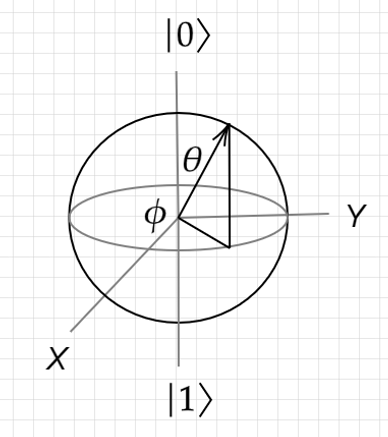
\includegraphics[scale = 0.7]{Bloch-Sphere.png}
		\caption{Bloch sphere representation of an arbitrary qubit state $\ket{\psi} = \cos(\theta/2)\ket{0} + e^{(i\phi)} \sin(\theta/2)\ket{1}$}
	\end{figure}
	On the Bloch Sphere, plot the following qubits (show a plot similar to a diagram above):
	\begin{parts}
		\part[2] \[\frac{\sqrt{3}}{2}\ket{0} + \frac{1}{2}\ket{1}\]
		\part[3] \[ \frac{1+i}{2}\ket{0} + \frac{1-i}{2}\ket{1}\]
	\end{parts}
	Next, consider the following operations:
	\[
		(i) \;\;	R(\theta_1) = \begin{bmatrix}
			\cos(\theta_1) & -\sin(\theta_1) \\
			\sin(\theta_1) & \cos(\theta_1)
		\end{bmatrix},
		(ii) \;\;	S(\phi_2) = \begin{bmatrix}
			1 & 0           \\
			0 & e^{i\phi_2}
		\end{bmatrix}\]

	Given an arbitrary qubit on the $X$-$Z$ plane (i.e.) its amplitudes have no imaginary component,

	\begin{parts}
		\part[2] what is the effect of applying $R(\theta_1)$ to it? In particular state the effect when $\theta_1 = \pi/2$?
		\part[3] what is the effect of applying $S(\phi_2)$ to it? In particular state the effect when $\phi_2 = \pi/2$?
	\end{parts}

	\begin{solution}

	\end{solution}

	\question[10] So far we have studied qubits defined using two basis states: $\ket{0}$ and $\ket{1}$. We have also seen two related states: the $\ket{+}$ state and the $\ket{-}$ state. Answer the following questions with reasons:

	\begin{parts}
		\part[2] Do the $\ket{+}$ state and the $\ket{-}$ state form a pair of orthonormal states?
		\part[2] Can the $\ket{+}$ state and the $\ket{-}$ state be used as the basis states?
		\part If the answer to the both (a) and (b) is Yes, express the following qubits as a linear combination of the $\ket{+}$ state and the $\ket{-}$ state:
		\begin{subparts}
			\subpart[2] $\ket{0}$,
			\subpart[2] $\ket{1}$,
			\subpart[2] an arbitrary qubit: $\ket{\psi} = \alpha \ket{0} + \beta \ket{1}$.
		\end{subparts}
	\end{parts}

	\begin{solution}

	\end{solution}

	\question[10] The Pauli Matrices are given by:

	\begin{align*}
		X = \sigma_x & = \begin{pmatrix}
			                 0 & 1 \\
			                 1 & 0
		                 \end{pmatrix} \\
		Y = \sigma_y & = \begin{pmatrix}
			                 0 & -i \\
			                 i & 0
		                 \end{pmatrix} \\
		Z = \sigma_z & = \begin{pmatrix}
			                 1 & 0  \\
			                 0 & -1
		                 \end{pmatrix}
	\end{align*}


	Show that the following relations hold:
	\vspace{2pt}
	\begin{parts}
		\part[3] $HX$ = $ZH$,
		\part[3] $HY$ = $-YH$,
		\part[3] $HZ$ = $XH$.
	\end{parts}
	where $H$ is the Hadamard operation.
	\vspace{2pt}

	\begin{parts}
		\part[1] Using these properties, show that $HXHYHZ = ZYXH$.
	\end{parts}

	\begin{solution}
		Lets first proof some results that we will use later on. First we will proof that \(H^\dagger = H\).
		\begin{proof}
			\label{HinveqH}
			\begin{align*}
				H^\dagger   & = \frac{1}{\sqrt{2}} \begin{pmatrix}
					                                   1 & 1  \\
					                                   1 & -1
				                                   \end{pmatrix}^\dagger          \\
				\iff \qquad & = \frac{1}{\sqrt{2}} \left(\begin{pmatrix}
						                                         1 & 1  \\
						                                         1 & -1
					                                         \end{pmatrix}^*\right)^T \\
				\iff \qquad & = \frac{1}{\sqrt{2}} \begin{pmatrix}
					                                   1 & 1  \\
					                                   1 & -1
				                                   \end{pmatrix}^T                \\
				\iff \qquad & = \frac{1}{\sqrt{2}} \begin{pmatrix}
					                                   1 & 1  \\
					                                   1 & -1
				                                   \end{pmatrix}                 \\
				\iff \qquad & = H
			\end{align*}
			This shows that \(H^{-1}=H\).
		\end{proof}
		Lets prove \(HX=ZH\),
		\begin{proof}
			\begin{align*}
				HX          & = \frac{1}{\sqrt{2}} \begin{pmatrix}
					                                   1 & 1  \\
					                                   1 & -1
				                                   \end{pmatrix} \begin{pmatrix}
					                                                 0 & 1 \\
					                                                 1 & 0
				                                                 \end{pmatrix} \\
				\iff \qquad & = \frac{1}{\sqrt{2}} \begin{pmatrix}
					                                   1  & 1 \\
					                                   -1 & 1
				                                   \end{pmatrix}               \\
				\iff \qquad & = \frac{1}{\sqrt{2}} \begin{pmatrix}
					                                   1 & 0  \\
					                                   0 & -1
				                                   \end{pmatrix} \begin{pmatrix}
					                                                 1 & 1  \\
					                                                 1 & -1
				                                                 \end{pmatrix} \\
				\iff \qquad & =  \begin{pmatrix}
					                 1 & 0  \\
					                 0 & -1
				                 \end{pmatrix} \frac{1}{\sqrt{2}}\begin{pmatrix}
					                                                 1 & 1  \\
					                                                 1 & -1
				                                                 \end{pmatrix} \\
				\iff \qquad & = ZH
			\end{align*}
		\end{proof}
		Now we will prove \(HY=-YH\),
		\begin{proof}
			\begin{align*}
				HY          & = \frac{1}{\sqrt{2}} \begin{pmatrix}
					                                   1 & 1  \\
					                                   1 & -1
				                                   \end{pmatrix} \begin{pmatrix}
					                                                 0 & -i \\
					                                                 i & 0
				                                                 \end{pmatrix} \\
				\iff \qquad & = \frac{1}{\sqrt{2}} \begin{pmatrix}
					                                   i  & -i \\
					                                   -i & -i
				                                   \end{pmatrix}               \\
				\iff \qquad & = \frac{1}{\sqrt{2}} \begin{pmatrix}
					                                   0 & -i \\
					                                   i & 0
				                                   \end{pmatrix} \begin{pmatrix}
					                                                 1 & 1  \\
					                                                 1 & -1
				                                                 \end{pmatrix} \\
				\iff \qquad & =  \begin{pmatrix}
					                 0 & -i \\
					                 i & 0
				                 \end{pmatrix} \frac{1}{\sqrt{2}}\begin{pmatrix}
					                                                 1 & 1  \\
					                                                 1 & -1
				                                                 \end{pmatrix} \\
				\iff \qquad & = -YH
			\end{align*}
		\end{proof}
		Now we will prove \(HZ=XH\),
		\begin{proof}
			We have proved that \(HX=ZH\), and we also know that \(H^{-1}=H\). So,
			\begin{align*}
				ZH              & = HX       \\
				\iff  H^{-1}ZH  & = H^{-1}HX \\
				\iff  HZH       & = X        \\
				\iff  HZHH^{-1} & = XH^{-1}  \\
				\iff  HZ        & = XH
			\end{align*}
		\end{proof}
		For the last part,
		\begin{proof}
			\begin{align*}
				HXHYHZ                 & = (HX)HY(HZ) \\
				\iff\qquad\qquad\qquad & = (ZH)HY(XH) \\
				\iff\qquad\qquad\qquad & = Z(HH)YXH   \\
				\iff\qquad\qquad\qquad & = Z(I)YXH    \\
				\iff\qquad\qquad\qquad & = ZYXH
			\end{align*}
		\end{proof}
	\end{solution}

	\question[10] We have seen earlier that if we are given one of the two quantum states $\ket{+}$ and $\ket{-}$ such that it is not known whether it is a $\ket{+}$ and $\ket{-}$, we can distinguish between them \textit{perfectly} by applying a Hadamard operation followed by a measurement.


	Suppose we are randomly sent one of the following two states:
	\begin{enumerate}[(a)]
		\item \(\displaystyle \frac{1}{2}\ket{0} + \frac{\sqrt{3}}{2}\ket{1}\)
		\item \(\displaystyle \frac{\sqrt{3}}{2}\ket{0} - \frac{1}{2}\ket{1}\)
	\end{enumerate}

	Devise a procedure to find out which one of the two states has been sent that performs better than a random choice. More specifically, given one of the two qubits, by performing your operation(s) followed by a measurement, the probability of finding out which one of the states is greater than random guessing i.e. greater than 1/2.

	\begin{solution}

	\end{solution}


\end{questions}

\end{document}